\section{Method Details}\label{app:method}
\paragraph{Training schedule.} We train with AdamW~\cite{loshchilov2019decoupled} (weight decay $10^{-4}$, batch size 32) and a one-cycle schedule~\cite{smith2019super} (peak learning rate $3\times10^{-3}$ for the heads and $3\times10^{-4}$ for the backbone, 10\% warm-up, then cosine decay) for up to 180 epochs, stopping early after 25 epochs without a lower validation loss, with gradient clipping at 1.0, mixed precision and seed 42. Training took 1\,h\,40\,min on one NVIDIA Tesla T4 (47\,s per epoch). Early stopping ended it after 125 epochs, before the one-cycle schedule had completed; the reported checkpoint, the one with the lowest validation loss, is from epoch 100. Every run in this paper uses the same stopping rule, but runs stop at different epochs, which we take into account when comparing them. The model is exported to ONNX (opset 17, which bilinear grid sampling requires) and to FP16.

\subsection{Augmentation}\label{app:aug}
Besides the distractor pasting of Section~\ref{sec:ownership}, we use horizontal flips (but no vertical flips, because a wearer's hand entering from the top would contradict the ownership prior), shift, scale and rotation, perspective warps, brightness and contrast changes, Gaussian blur, and mixup~\cite{zhang2018mixup} between images of the same scene. With probability 0.15, we also paste an unlabelled patch that contains no hand, so that a pasted rectangle is not itself a cue. In the hand-heatmap loss, the negative term near a pasted hand is multiplied by $1+4\,G_k$, where $G_k$ is a Gaussian ($\sigma{=}1.5$ cells) at that hand's centre. Table~\ref{tab:aug} lists all settings.

\begin{table}[h]
  \caption{Training-time augmentation, applied on the fly; each training image is seen once per epoch as a new random variant. Validation and test images are only resized and normalised.}
  \label{tab:aug}
  \footnotesize
  \begin{tabular}{lp{0.62\linewidth}}
    \toprule
    Step & Setting \\
    \midrule
    Distractor hands & 1--2 hands with probability 0.5 (hand images) or 0.3 (no-hand images); scale 0.45--1.0; rotation by 90/180/270$^\circ$ and optional mirror with probability 0.7; centre in the top 65\% of the frame; overlap with the wearer's hand and the target below 15\%; feathered alpha (12\% of the crop size); colour jitter; 30\% self-paste; pool of 512 donor crops, half from pointing hands \\
    Decoy patch & unlabelled non-hand patch from a no-hand image, with probability 0.15 \\
    Horizontal flip & 0.5 \\
    Shift / scale / rotate & ${\pm}5\%$ / ${\pm}10\%$ / ${\pm}15^\circ$, probability 0.4 \\
    Perspective & scale 0.02--0.05, probability 0.2 \\
    Brightness / contrast & ${\pm}20\%$, probability 0.5 \\
    Gaussian blur & kernel 3--5, probability 0.2 \\
    Mixup & within the same scene, $\lambda\sim\mathrm{Beta}(0.2,0.2)$ folded to ${\geq}0.5$, label of the dominant image, every batch \\
    Anchor forcing & ground-truth anchors with probability 0.5 decaying to 0 over 20 epochs \\
    \bottomrule
  \end{tabular}
\end{table}

\section{Data}\label{app:data}

\paragraph{EgoPoint.} The EgoPoint-Ground paper~\cite{egopoint} reports 15,338 images: 39\% (6,035) real captures with smart glasses, 39\% (5,976) synthetically composed and 22\% (3,327) generated by editing; its appendix calls the last two groups ``synthetic generation'' and ``image editing''. The edited images were made from third-person photographs of COCO~\cite{lin2014coco}, selected through the RefCOCO referring-expression dataset~\cite{yu2016modeling}, into which a multimodal model added a pointing hand. The release we use has 15,455 images split 10,837 / 1,546 / 3,072. VistaRef~\cite{li2026vistaref} and PointVG-R~\cite{li2026pointvgr} report the same counts, so our test images are theirs, minus the exclusions below. Each positive record shows one wearer's hand pointing at one target; negatives show no hand.

\paragraph{Conversion.} Negatives become scene 000 (no hand), and their object boxes are ignored; positives with a hand box, an annotated fingertip and a target box become scene 111 (pointing at a target). In three test records, the hand label was attached to an object and the hand was labelled as an object; we detected these by the fingertip position and swapped the labels back. We dropped 232 positives: 229 without an annotated fingertip (164 train, 22 validation, 43 test), all flagged as unclear in the source annotations, and 3 without a hand box. Spot checks showed open palms, held objects, or a hand box on the hand that was not pointing. If all 43 dropped test positives were counted as failures, the target P@0.5 would fall by less than one point, to about 58\%. Images are stored at $224\times224$; the model squashes every frame to its square $160\times160$ input, regardless of the original aspect ratio. Table~\ref{tab:data} summarises the result.

\paragraph{Fingertip--target gap.} We describe each target by its gap to the fingertip in the image: \emph{overlap} when the fingertip lies inside the target box, \emph{near} when the shortest fingertip--box distance is at most 0.08 of the image side, and \emph{large gap} otherwise. These are image-plane relations: an overlap does not imply that the finger touches the object, and a large gap does not imply that the object is far from the wearer. About 70\% of targets overlap the fingertip and only 7\% have a large gap, so pooled results are dominated by overlap targets; Appendix~\ref{app:heads} reports the main metrics by gap.

\begin{table}[h]
  \caption{EgoPoint after conversion, by split, scene and fingertip--target gap.}
  \label{tab:data}
  \footnotesize
  \begin{tabular}{lrrrrrr}
    \toprule
    & & & & \multicolumn{3}{c}{Pointing at target, by gap} \\
    \cmidrule(l){5-7}
    Split & Images & No hand (000) & Pointing at target (111) & Overlap & Near & Large gap \\
    \midrule
    Train & 10,669 & 1,535 & 9,134 & 6,511 & 1,995 & 628 \\
    Validation & 1,524 & 211 & 1,313 & 922 & 297 & 94 \\
    Test & 3,029 & 425 & 2,604 & 1,796 & 599 & 209 \\
    \midrule
    Total & 15,222 & 2,171 & 13,051 & 9,229 & 2,891 & 931 \\
    \bottomrule
  \end{tabular}
\end{table}

\paragraph{COCO overlap.} The release names the source photograph of each edited image. In our test split, 842 of the 2,604 images with a target (32\%) are edited COCO train2014 photographs, and at least 400 of the 425 no-hand images are unedited COCO train2014 photographs, so at least 1,242 test images (41\%) come from COCO. COCO-pretrained detector weights are trained on COCO train2017, which contains every train2014 photograph, together with box annotations of the objects they contain. In addition, 230 test images share their COCO source photograph with a training or validation image; this overlap within EgoPoint affects all trained models alike.

\paragraph{Near-duplicates.} 141 test images (4.7\%) are byte-identical to a training or validation image, and 362 have an exact or near copy there. We therefore repeat the headline comparisons on the test split without the 141 duplicates. Unless stated otherwise, every conclusion holds on that duplicate-free set; the main model's P@0.5 moves from 58.9\% to 57.2\%, inside its confidence interval.

\paragraph{Model selection.} Training, early stopping and checkpoint selection use only the training and validation splits; the test split is evaluated once, after training. The ablation, resolution and seed runs follow the same rule and do not change the reported model.

\section{Additional Results}\label{app:extra}

\subsection{Comparison with Published Models and the Benchmark Detectors}\label{app:comparison}

Table~\ref{tab:main-full} extends Table~\ref{tab:main}. VistaRef and PointVG-R report results on the same 3,072-image test split, from which ours omits 43 unclear images and the 425 images without a target; PointVG-R also reports zero-shot and fine-tuned multimodal LLMs on that split. EgoPoint-Ground's pointing-only (POG) results come from a different setting: zero-shot models receive the ground-truth hand box, and the evaluated subset is not stated. Three simple references test whether knowing where the fingertip is would be enough: the mean training target box at a fixed position, and a box of mean training size centred on SpatialNet's predicted fingertip or on the ground-truth fingertip. A mean-size box at the true fingertip reaches a P@0.5 of only 11.4\% (12.0\% when shifted by the mean training offset), because target sizes vary widely (2.6\% to 44\% of the image area, 10th to 90th percentile).

Against zero-shot multimodal LLMs the picture is mixed. SpatialNet's P@0.5 and mIoU are above those reported for zero-shot Qwen2.5-VL-7B and Qwen3-VL-8B, and its P@0.3 is far higher, but the zero-shot models draw tighter boxes (P@0.7 of 39.0--42.9\% against 31.8\%), and models given the true hand box reach 61.2--63.9\% P@0.5. Because the published rows count IoU${>}\tau$, include no-target images scored in an unstated way and, in one case, use an unstated subset, and because models trained on large image collections may also have seen COCO, we read this as the same accuracy range at a fraction of the size, not as parity or superiority.

\begin{table}[h]
  \caption{Localisation of the pointed-at target on the EgoPoint test split. Our rows use the 2,604 test images with a target. mIoU and P@$\tau$ in \%, the published values multiplied by 100. We count IoU${\geq}\tau$, as does VistaRef; EgoPoint-Ground and PointVG-R count IoU${>}\tau$. \emph{Large gap}: P@0.5 on the 209 large-gap targets.
  $^\ast$\,VistaRef~\cite{li2026vistaref}, Table~1, setting ``Train-Real Data Test'', BEiT-3-L backbone (226M parameters with BEiT-3-Base); test set of 3,072 images, which includes no-hand images.
  $^\ddagger$\,PointVG-R~\cite{li2026pointvgr}, Table~1, EgoPoint-CoT test set, built on the same release and test split.
  $^\dagger$\,EgoPoint-Ground~\cite{egopoint}, Table~4, pointing-only (POG) task: inference only, given the ground-truth hand box; the evaluated subset is not stated.
  How the published works score images without a target is not stated; if they counted the 425 no-target images as failures, zero-shot Qwen2.5-VL-7B would reach about 57.8\% P@0.5 and 52.8\% mIoU on the images with a target.}
  \label{tab:main-full}
  \footnotesize
  \setlength{\tabcolsep}{3.4pt}
  \begin{tabular}{lrrrrrr}
    \toprule
    Method & Params & P@0.3 & P@0.5 & P@0.7 & mIoU & Large gap \\
    \midrule
    \multicolumn{7}{l}{\emph{Published, trained on EgoPoint (not re-run)}} \\
    \quad VistaRef$^\ast$, image + fixed prompt & $>$226M & 97.0 & 93.9 & 82.6 & 82.0 & -- \\
    \quad PointVG-R$^\ddagger$, image + instruction, SFT + RL & 7B & 88.1 & 83.6 & 74.5 & 75.7 & -- \\
    \quad Qwen2.5-VL-7B$^\ddagger$, image + instruction, SFT & 7B & 68.7 & 63.6 & 56.7 & 59.8 & -- \\
    \multicolumn{7}{l}{\emph{Published, zero-shot (not re-run)}} \\
    \quad Qwen2.5-VL-7B$^\ddagger$, image + instruction & 7B & 54.2 & 49.8 & 42.9 & 45.5 & -- \\
    \quad Qwen3-VL-8B$^\ddagger$, image + instruction & 8B & 48.1 & 44.5 & 39.0 & 43.0 & -- \\
    \quad SV-CoT$^\dagger$, image + hand box & $>$1B & 69.4 & 63.9 & 55.6 & -- & -- \\
    \quad Qwen3-VL-4B$^\dagger$, image + hand box & 4B & 67.1 & 61.2 & 53.2 & -- & -- \\
    \multicolumn{7}{l}{\emph{Simple references}} \\
    \quad Mean training box, fixed position & 0 & 41.3 & 9.6 & 0.9 & 27.4 & 4.3 \\
    \quad Mean-size box at predicted fingertip & 0.72M & 43.5 & 11.2 & 0.9 & 28.8 & 0.0 \\
    \quad Mean-size box at true fingertip (oracle) & -- & 43.6 & 11.4 & 1.0 & 29.0 & 0.0 \\
    \midrule
    \textbf{SpatialNet} (image only, seed 42) & 0.72M & 78.6 & 58.9 & 31.8 & 53.3 & 25.4 \\
    \quad mean $\pm$ std, 3 seeds & & 78.1{\scriptsize$\pm$0.6} & 59.0{\scriptsize$\pm$0.1} & 31.5{\scriptsize$\pm$0.4} & 52.9{\scriptsize$\pm$0.5} & 26.3{\scriptsize$\pm$1.3} \\
    \bottomrule
  \end{tabular}
\end{table}

\paragraph{Benchmark of compact detectors.} Table~\ref{tab:detectors} compares SpatialNet with YOLO26n and NanoDet-Plus-m from several starting points, trained on the same split and scored with the same code, plus higher-resolution runs of both. \tbd{State the benchmark detectors' training recipe: classes, epochs, augmentation, how one hand box and one target box are selected per image, and the validation rule used to tune the hand-gate thresholds of the end-to-end score.} GFLOPs are counted with the same \texttt{torch} FLOP counter; model sizes are the serialised SpatialNet state dicts and the exported ONNX files of the detectors, of which we count only the inference parameters. With the same ImageNet pretraining as our backbone, YOLO26n is 4.3 points ahead in P@0.5, mostly in tight boxes (P@0.7 +10.6) and large-gap targets (+11.4), and its hand mIoU is 7.4 points higher; trained from scratch, it is 1.0 point ahead.

\paragraph{End-to-end score.} The target metrics ignore the gates. The end-to-end score covers all 3,029 test images: a target image counts as correct if the hand gate fires, the model predicts ``pointing at target'' and the target box has IoU${\geq}0.5$; a no-hand image counts as correct if the model says ``no hand''. Each model's hand-gate threshold is tuned on the validation split by the same rule. Counting the gate costs each model 0.3--1.3 points of P@0.5, and every model rejects 95.3--98.4\% of no-hand frames, so the order does not change: SpatialNet reaches 63.6\%, on a par with YOLO26n from scratch (63.8\%) and below YOLO26n with an ImageNet start (67.4\%) and the COCO-pretrained detectors (68.9--71.1\%). On the test split without duplicates the order is the same.

\begin{table}[h]
  \caption{SpatialNet and the benchmark detectors, trained on EgoPoint and scored by the same code (\%, on the 2,604 test images with a target, except \emph{End-to-end}, which covers all 3,029 test images). \emph{Pasted}: change in target P@0.5 when one or two hands are pasted into each test image; none of these detectors was trained with pasted hands. $^\dagger$\,Pretrained on COCO train2017.}
  \label{tab:detectors}
  \footnotesize
  \setlength{\tabcolsep}{3pt}
  \begin{tabular}{lrrrrrrrrrr}
    \toprule
    Model & Params & GFLOPs & P@0.5 & P@0.7 & mIoU & Large & Hand & Centre & Pasted & End-to- \\
    & & & & & & gap & mIoU & in & & end \\
    \midrule
    \multicolumn{11}{l}{\emph{Matched compute}} \\
    SpatialNet, 160\,px, ImageNet & 0.72M & 0.231 & 58.9 & 31.8 & 53.3 & 25.4 & 73.7 & 84.8 & $+$1.2 & 63.6 \\
    YOLO26n, 128\,px, scratch & 2.50M & 0.225 & 59.9 & 39.1 & 54.7 & 31.6 & 80.6 & 81.6 & $-$4.6 & 63.8 \\
    YOLO26n, 128\,px, ImageNet & 2.50M & 0.225 & 63.2 & 42.4 & 56.8 & 36.8 & 81.1 & 82.3 & $-$3.6 & 67.4 \\
    YOLO26n, 128\,px, COCO$^\dagger$ & 2.50M & 0.225 & 65.0 & 47.0 & 58.6 & 39.7 & 81.6 & 82.2 & $-$4.0 & 68.9 \\
    NanoDet-Plus-m, 160\,px, COCO$^\dagger$ & 1.17M & 0.218 & 67.6 & 49.5 & 59.8 & 40.7 & 81.5 & 82.9 & $-$4.5 & 71.1 \\
    \midrule
    \multicolumn{11}{l}{\emph{Higher compute}} \\
    SpatialNet, 224\,px, ImageNet & 0.72M & 0.453 & 62.4 & 37.1 & 54.8 & 35.9 & 74.9 & 83.7 & $+$1.5 & 66.8 \\
    SpatialNet, 320\,px, ImageNet & 0.72M & 0.923 & 65.1 & 40.3 & 56.5 & 34.9 & -- & -- & -- & 69.3 \\
    YOLO26n, 160\,px, COCO$^\dagger$ & 2.50M & 0.352 & 66.9 & 48.8 & 60.3 & 42.1 & 82.1 & 83.5 & $-$3.0 & 70.8 \\
    YOLO26n, 192\,px, COCO$^\dagger$ & 2.50M & 0.507 & 69.9 & 53.3 & 62.8 & 43.5 & 82.9 & 84.7 & $-$2.6 & 73.6 \\
    \bottomrule
  \end{tabular}
\end{table}

\subsection{Controlled Detector Runs}\label{app:controlled}

We trained YOLO26n ourselves under one fully specified recipe (Ultralytics 8.4.177): the converted EgoPoint images at $128\times128$; two classes, the wearer's hand and the target, with no labels on no-hand images; 150 epochs with early stopping after 50 epochs without improvement, batch 64; and Ultralytics' default augmentation without mosaic, mixup or copy-paste. The backbone starts from ImageNet (the YOLO26n classification weights, which initialise its first ten layers, with the neck and head from scratch) or from COCO. One ImageNet-start run is also trained with our distractor pasting, applied on the fly with the same code and probabilities as for SpatialNet; the pasted hands stay unlabelled background, since a detector has no ownership-weighted heatmap loss. For each image we score the top-scoring hand box and target box, and for every model, SpatialNet included, the hand-gate threshold is the value that maximises no-hand versus hand accuracy on the validation split (Table~\ref{tab:controlled}).

The ImageNet-start run reproduces the benchmark (62.9\% against 63.2\% P@0.5), and its second seed differs from it by 0.6 points ([$-$1.0, +2.2]). Against the first seed, SpatialNet is 4.0 points lower in P@0.5 ([$-$6.0, $-$2.2]) and 11.6 lower in P@0.7 ([$-$13.4, $-$9.6]); against the second, 4.6 and 11.5 points lower. Its predicted target centre lies inside the labelled box more often than for every run: the paired differences are 2.8 [1.4, 4.1] and 3.2 [1.8, 4.6] points against the two ImageNet-start seeds, 3.0 [1.7, 4.5] against the run with pasting and 2.6 [1.3, 4.0] against the COCO start.

\paragraph{Robustness to other hands comes from the training recipe.} Trained without pasting, the detectors lose 2.4--4.1 points of P@0.5 when hands are pasted into the test images and keep only 87.8--88.7\% of no-hand frames, whereas SpatialNet gains 1.2 points and keeps 96.7\%. Trained with our pasting, the same YOLO26n is as stable as SpatialNet: it changes by $+$0.7 points (difference from SpatialNet $-$0.6 [$-$2.2, $+$0.8]) and keeps 95.8\% of no-hand frames ($-$0.9 [$-$3.8, $+$1.4]). Pasting improves the detector's change under interference by 3.8 points [2.4, 5.2] and the no-hand frames kept by 8.0 [5.2, 10.8], at no cost on clean images (P@0.5 $+$0.3 [$-$1.2, $+$1.8]).

\paragraph{COCO pretraining does not exploit the overlap.}\label{app:coco} If COCO pretraining helped mainly by having seen the test sources, its gain would concentrate on the 842 COCO-derived test images. It does the opposite: against the ImageNet start, the COCO start gains 2.4 points [0.6, 4.3] on the other test images and $-$0.7 [$-$3.7, $+$2.5] on the COCO-derived ones (difference $-$3.2 [$-$6.7, $+$0.3]). NanoDet-Plus-m was not retrained, so this test covers YOLO26n only. All models, SpatialNet included, find the COCO-derived images harder (51.8--56.1\% against 62.3--68.7\% P@0.5).

\begin{table}[h]
  \caption{SpatialNet and four controlled YOLO26n runs (128\,px), scored by the same code on the same test images (\%). \emph{Pasted}: change in target P@0.5 with one or two pasted hands per image. \emph{No hand kept}: no-hand images still classed as no hand when hands are pasted into them, at validation-tuned thresholds. \emph{COCO} and \emph{Other}: P@0.5 on the 842 test images made from COCO train2014 photographs and on the remaining 1,762.}
  \label{tab:controlled}
  \footnotesize
  \setlength{\tabcolsep}{2.6pt}
  \begin{tabular}{lrrrrrrrrr}
    \toprule
    & & & Large & Hand & Centre & & No hand & \multicolumn{2}{c}{P@0.5, source} \\
    \cmidrule(l){9-10}
    Model & P@0.5 & P@0.7 & gap & mIoU & in & Pasted & kept & COCO & Other \\
    \midrule
    \textbf{SpatialNet} (ImageNet) & 58.9 & 31.8 & 25.4 & 73.7 & \textbf{84.8} & $+$1.2 & 96.7 & 51.8 & 62.3 \\
    YOLO26n, ImageNet & 62.9 & 43.4 & 36.8 & 81.0 & 82.1 & $-$3.1 & 87.8 & 56.1 & 66.2 \\
    YOLO26n, ImageNet, seed 1 & 63.6 & 43.3 & 38.3 & 81.0 & 81.6 & $-$4.1 & 88.7 & 54.9 & 67.7 \\
    YOLO26n, ImageNet + pasting & 63.2 & 42.7 & 36.8 & 80.9 & 81.8 & $+$0.7 & 95.8 & 55.5 & 66.9 \\
    YOLO26n, COCO & 64.4 & 45.5 & 36.4 & 81.4 & 82.2 & $-$2.4 & 87.8 & 55.3 & 68.7 \\
    \bottomrule
  \end{tabular}
\end{table}

\paragraph{Ownership under pasted hands.} With one or two hands pasted into each test image (Table~\ref{tab:own}), SpatialNet's hand lies nearer the wearer's hand than any pasted hand in 99.7\% of hand images, and its target P@0.5 does not drop. This ownership metric is easy under the synthetic distribution: pasted hands sit in the upper part of the frame and the wearer's hand in the lower part, so ownership accuracy on training batches was already 93\% in the first epoch. The no-hand frames kept and the target accuracy under interference are more informative, and both need the pasting recipe (ablation A1).

\begin{table}[h]
  \caption{Ownership on test images with one or two pasted hands (\%). \emph{On other hand}: predicted hand centre inside a pasted hand. \emph{No hand kept}: no-hand images still classed as no hand, at the hand-gate threshold of 0.5.}
  \label{tab:own}
  \footnotesize
  \begin{tabular}{lrrrr}
    \toprule
    & Ownership accuracy & On other hand & No hand kept & Target P@0.5 \\
    \midrule
    Full model, clean test images & -- & -- & 93.4 & 58.9 \\
    Full model, pasted hands & 99.7 [99.4, 99.9] & 0.2 & 91.8 & 60.1 \\
    A1 (no pasting), pasted hands & 98.7 [98.2, 99.1] & 1.2 & 86.4 & 56.1 \\
    \bottomrule
  \end{tabular}
\end{table}

\subsection{Per-Head Accuracy and Hand Presence}\label{app:heads}

\begin{table}[h]
  \caption{Accuracy of each head by fingertip--target gap (test split, pointing-at-target images). Fingertip error in pixels at the $160\times160$ input; direction error in degrees. mIoU and P@0.5 in \%; brackets: 95\% bootstrap confidence intervals of the mIoU.}
  \label{tab:heads}
  \footnotesize
  \setlength{\tabcolsep}{4pt}
  \begin{tabular}{lrrrrrrrr}
    \toprule
    & \multicolumn{2}{c}{Hand} & \multicolumn{2}{c}{Fingertip (px)} & \multicolumn{2}{c}{Direction ($^\circ$)} & \multicolumn{2}{c}{Target} \\
    \cmidrule(lr){2-3}\cmidrule(lr){4-5}\cmidrule(lr){6-7}\cmidrule(l){8-9}
    Gap (images) & mIoU & P@0.5 & mean & ${<}5$\,px & mean & ${<}15^\circ$ & mIoU [CI] & P@0.5 \\
    \midrule
    Overlap (1,796) & 73.7 & 92.3 & 3.79 & 84.4 & 36.0 & 39.7 & 57.9 [56.8, 59.0] & 66.0 \\
    Near (599) & 73.7 & 93.5 & 4.09 & 78.8 & 22.0 & 54.9 & 47.8 [45.8, 49.8] & 49.2 \\
    Large gap (209) & 72.7 & 92.8 & 4.16 & 80.9 & 29.0 & 36.8 & 29.8 [26.0, 33.6] & 25.4 \\
    \midrule
    All (2,604) & 73.7 & 92.6 & 3.89 & 82.8 & 32.2 & 43.0 & 53.3 [52.3, 54.3] & 58.9 \\
    \bottomrule
  \end{tabular}
\end{table}

\paragraph{Where the errors come from.} The hand box and fingertip are equally good at every gap (hand P@0.5 of 92--94\%; about 4\,px fingertip error, 2.5\% of the image side), so they are not the bottleneck. The target falls off with the gap: P@0.5 drops from 66.0\% for overlap targets to 49.2\% for near and 25.4\% for large-gap ones (Table~\ref{tab:heads}). The direction is coarse: its median error is 18.6$^\circ$, and only 36.8\% of large-gap targets have an error below 15$^\circ$. At their median fingertip--target distance of 0.32 image widths, 15$^\circ$ already moves the ray by about 0.08 image widths, the size of a small object. The error is largest for overlap targets (36$^\circ$), where the direction to the target centre is ill-defined and matters least. Position and extent errors contribute about equally: giving the model the true size with its own centre would raise P@0.5 to 70.4\%, and giving it the true centre with its own size would raise it to 72.3\%. Size is regressed towards the mean: small targets (under 3\% of the image) are predicted about 1.9 times too large and reach a P@0.5 of only 36.9\% (27.8--36.9\% across seeds).

\paragraph{Hand presence.} The hand gate separates no-hand from pointing frames with 98.6\% accuracy (95\% CI 98.1--98.9) and AUROC 0.998. At threshold 0.5, it misses 15 of 2,604 hands (0.6\%) and raises false alarms on 28 of 425 no-hand frames (6.6\%). Choosing the threshold on validation so that no hand is missed (0.22) would raise false alarms to 117 (27.5\%), so we keep 0.5. Per-frame false alarms of this size mean that an always-on interface needs temporal smoothing, for example requiring several consecutive detections, which we do not evaluate.

\subsection{Recognition Test}\label{app:recog}

\paragraph{Protocol.} For each of the 2,603 test targets with a category name, we crop the predicted target box of each model from the 320\,px copy of the image, restore the photograph's original aspect ratio, pad the crop to a square and classify it zero-shot among the 348 target category names of EgoPoint, averaging four prompt templates (``a photo of a \{\}.'' and three variants). Crops of the labelled box and of the whole frame are references. The test is category-level: a box on a neighbouring object of the same category counts as recognised, and near-synonyms such as ``bike'' and ``bicycle'' count as errors, for every model alike. Both recognisers ran on CPU; larger recognisers (CLIP ViT-L/14, SigLIP so400m) were planned on a GPU, but those runs did not complete.

\paragraph{Further results.} Top-5 accuracy gives the same result as top-1 (differences from $-$1.3 to 0.0 points; one interval of eight excludes zero, by 0.04 points), and so do SpatialNet's seeds 1 and 2 (48.3--49.1\% and 52.5--52.6\% top-1). When SpatialNet's box misses IoU 0.5 but its centre lies on the labelled object, the crop is still named correctly in 47--51\% of cases, against 54--58\% for boxes with IoU${\geq}0.5$ and 30\% when the centre misses. Large-gap targets are the exception (Table~\ref{tab:recog-full}): there, the detectors' crops are named correctly 4.3--8.1 points more often than those of the deployed model (the interval excludes zero in five of the eight comparisons; seeds 1 and 2 of SpatialNet lie in between, at 37.3--43.1\%), and its crops are named about as often as the whole frame, or less often. Restricting the test to targets other than people, 20\% of the test set, changes no difference by more than one point.

\begin{table}[h]
  \caption{Recognition test with the large-gap subset (top-1 accuracy, \%; 2,603 test targets, 209 of them with a large gap).}
  \label{tab:recog-full}
  \footnotesize
  \begin{tabular}{lrrrr}
    \toprule
    & \multicolumn{2}{c}{CLIP ViT-B/16} & \multicolumn{2}{c}{SigLIP base} \\
    \cmidrule(lr){2-3}\cmidrule(l){4-5}
    Crop & All & Large gap & All & Large gap \\
    \midrule
    Labelled box (upper reference) & 53.9 & 51.2 & 59.4 & 54.1 \\
    Whole frame (lower reference) & 40.3 & 33.5 & 46.2 & 43.1 \\
    \midrule
    \textbf{SpatialNet} (seed 42) & 48.6 & 34.9 & 52.3 & 36.8 \\
    YOLO26n, ImageNet & 48.8 & 43.1 & 53.3 & 41.6 \\
    YOLO26n, ImageNet, seed 1 & 49.1 & 41.1 & 53.4 & 41.1 \\
    YOLO26n, ImageNet + pasting & 49.9 & 43.1 & 52.0 & 43.5 \\
    YOLO26n, COCO & 49.1 & 42.1 & 53.2 & 42.1 \\
    \bottomrule
  \end{tabular}
\end{table}

\subsection{Input Resolution}\label{app:resolution}

A convolutional network shares its filters across positions, so a larger input costs compute but no parameters. We retrained the unchanged model (722,104 parameters, same seed and settings) at 224\,px, using the stored $224\times224$ images at full resolution instead of downsampling them, and at 320\,px, re-converting the dataset from the original images so that the larger input carries real detail rather than upsampled pixels (Table~\ref{tab:detectors}). From 160 to 320\,px, P@0.5 rises by 6.2 points (95\% paired-bootstrap CI [+4.4, +8.0]) to 65.1\%, P@0.7 by 8.5 points [+6.8, +10.3] and mIoU by 3.2, and the fingertip error falls from 2.43\% to 1.32\% of the image width; 224\,px lies in between. Large-gap targets gain first and then stop (25.4\% at 160\,px, 35.9\% at 224\,px, 34.9\% at 320\,px), while the mean direction error is flat at every resolution (31.4--32.2$^\circ$). With one run per resolution, this suggests, but does not show, that the direction estimate rather than the input limits large-gap targets beyond 224\,px. Small targets gain only at 320\,px (36.9\% $\to$ 46.6\% P@0.5), where the images were re-converted from the originals. Both higher-resolution runs stopped early at 84 epochs (best epoch 59, against 100 at 160\,px), so their gains may be underestimated. Compute grows from 0.23 to 0.45 and 0.92 GFLOPs (CPU latency on the evaluation machine 25.7, 37.2 and 50.8\,ms), while the weights stay at 1.6\,MB.

\subsection{Ablations}\label{app:ablation}

We retrain the 160\,px model without one component at a time, with the seed and settings of the main run: \textbf{A1} no distractor pasting and no ownership weighting; \textbf{A2} no geometric consistency terms; \textbf{A3} no ray conditioning of the target head (no $G^t$; 13,105 fewer parameters); \textbf{A4} no instance-anchored chain, so that the direction head and gates read the globally pooled vector and the fingertip has no hand-anchored terms, which gives a plain model of the same size (709K parameters). Each ablation was trained once, and we test each difference in two ways: a paired bootstrap over test images gives a 95\% interval for test-sample variation, and retraining the full model with two more seeds gives the training variation. A difference counts as an effect only if its interval excludes zero \emph{and} it exceeds the largest change that retraining alone produced (Table~\ref{tab:ablation-full}, second row). With one seed per variant and several metrics per component, we treat these comparisons as exploratory. Figure~\ref{fig:ablation} shows, for each component, the metrics it was designed to improve.

\begin{table}[h]
  \caption{Ablations at 160\,px, all metrics (one seed each). First row: the full model; other rows: difference from it (points, or degrees for the direction error, where positive means worse). Bold: the 95\% paired interval excludes 0 and the difference exceeds the retraining row. $^\S$\,Not significant on the duplicate-free test split. \emph{Small}: targets under 3\% of the image (309 images).}
  \label{tab:ablation-full}
  \footnotesize
  \setlength{\tabcolsep}{3pt}
  \begin{tabular}{lrrrrrrrrr}
    \toprule
    & \multicolumn{7}{c}{Clean test images} & \multicolumn{2}{c}{With other hands} \\
    \cmidrule(lr){2-8}\cmidrule(l){9-10}
    Variant & mIoU & P@0.5 & P@0.7 & Large gap & Small & Hand & Dir.\,($^\circ$) & P@0.5 & No hand \\
    \midrule
    Full model & 53.3 & 58.9 & 31.8 & 25.4 & 36.9 & 73.7 & 32.2 & 60.1 & 91.8 \\
    \quad Retraining (seeds 1, 2) & $\pm$0.9 & $\pm$0.1 & $\pm$0.8 & $\pm$2.4 & $\pm$9.1 & $\pm$0.3 & $\pm$1.2 & $\pm$0.4 & $\pm$3.3 \\
    \midrule
    A1 no hand pasting & \textbf{$-$1.2} & $-$0.1 & $-$1.3 & $+$1.9 & $-$3.9 & \textbf{$-$0.6} & \textbf{$+$1.8} & \textbf{$-$4.1} & \textbf{$-$5.4} \\
    A2 no ray / axis losses & $-$0.5 & $+$1.1 & $+$0.6 & $+$3.3 & $-$0.6 & $-$0.4 & \textbf{$+$1.5} & 0.0 & $-$1.2 \\
    A3 no ray conditioning & $+$0.2 & $+$0.7 & \textbf{$+$1.9}$^\S$ & $+$5.3 & $+$1.0 & 0.0 & \textbf{$-$1.3} & $+$1.0 & $+$1.2 \\
    A4 no anchor chain & \textbf{$-$1.4} & $-$0.3 & \textbf{$-$2.8}$^\S$ & $+$0.5 & \textbf{$-$11.3} & \textbf{$-$1.8} & \textbf{$+$3.4} & $-$0.5 & 0.0 \\
    \bottomrule
  \end{tabular}
\end{table}

\begin{figure}[h]
  \centering
  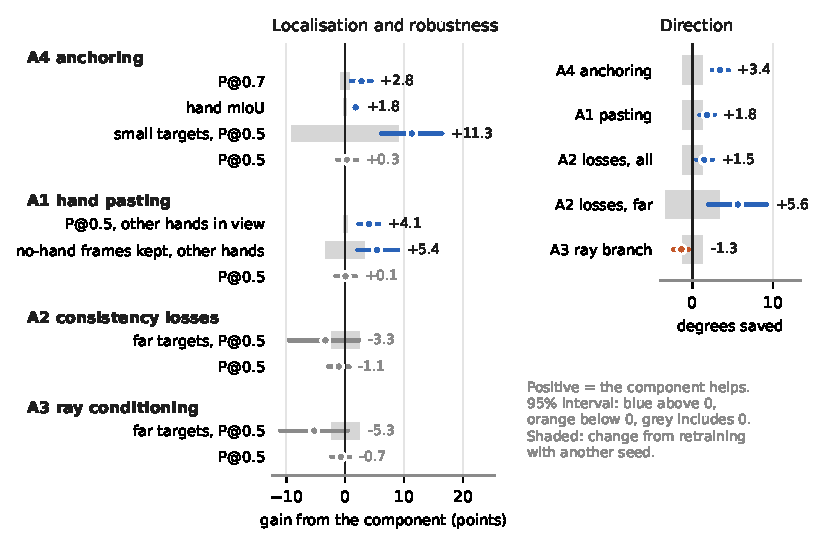
\includegraphics[width=\linewidth]{figures/ablation_effects}
  \caption{What each component contributes, with 95\% paired-bootstrap intervals. Gain = full model minus ablation, or degrees of direction error saved, so positive means the component helps. Grey bands: the largest change that retraining the full model with another seed produced on the same metric. ``Far'' in the labels denotes large-gap targets. The P@0.7 effect of A4 is not significant on the duplicate-free test split.}
  \Description{Interval plot with grey bands for retraining variation. Anchoring: P@0.7 +2.8, hand mIoU +1.8, small targets +11.3, all above zero and outside the bands; P@0.5 +0.3, crossing zero. Hand pasting: P@0.5 with other hands +4.1 and no-hand frames kept +5.4, above zero; P@0.5 +0.1. Consistency losses and ray conditioning: far-target and overall P@0.5 effects cross zero. Direction panel: degrees saved by anchoring 3.4, pasting 1.8, consistency losses 1.5 overall and 5.6 for far targets, all above zero; the ray branch -1.3, below zero.}
  \label{fig:ablation}
\end{figure}

\paragraph{A4, instance anchoring.} Against a plain model of the same size, the anchored chain improves hand mIoU by 1.8 points [+1.4, +2.2], against at most 0.3 between seeds, and lowers the direction error by 3.4$^\circ$ [2.4, 4.5], against at most 1.2$^\circ$. It also raises P@0.7 by 2.8 points [+1.1, +4.3] and small-target P@0.5 by 11.3 points [+6.5, +16.5] (the plain model's small boxes are drawn 2.4 instead of 1.9 times too large), but we treat these two as supporting evidence only: without duplicated test images the P@0.7 gain shrinks to 1.7 [0.0, +3.5], and the small-target gain is close to the seed spread (9.1). A4 also stopped earliest (best epoch 54, against 100), so its effects include a different training length.

\paragraph{A1, distractor pasting.} With other hands in view, the model trained with pasting keeps 4.1 more points of target P@0.5 [+2.4, +5.8] and 5.4 more points of no-hand frames as \emph{no hand} [+1.9, +8.9], and it puts its hand on another person's hand six times less often (0.2\% against 1.2\%). On clean images it costs nothing (P@0.5 $-$0.1) and even helps slightly (mIoU +1.2, hand mIoU +0.6, and 1.8$^\circ$ less direction error), which is consistent with pasting acting as a regulariser.

\paragraph{A2, consistency losses.} Without the two consistency terms, the direction error for large-gap targets rises by 5.6$^\circ$ [+2.1, +9.4], to 34.6$^\circ$, above all three seeds of the full model (29.0--32.3$^\circ$), and the overall direction error rises by 1.5$^\circ$, only slightly more than retraining alone changes it. Target-box accuracy does not change ($+$1.1 P@0.5, n.s.), because the target head does not draw on the predicted direction (A3). The losses therefore sharpen an output that an interface can use directly, for example to draw the pointing ray as feedback, but not the box.

\paragraph{Robustness of these conclusions.} Every difference reported above as an effect is significant under the paired bootstrap and larger than the change produced by retraining with another seed; effects close to that threshold (the small-target gain of anchoring, and the overall direction changes of A1--A3, 1.3--1.8$^\circ$ against 1.2$^\circ$) are supporting evidence only. Removing duplicated test images changes no conclusion except the P@0.7 effects of A3 and A4. The ablation variants stopped at different epochs (54 to 120), and some interventions are bundled (A1, A2 and A4).

\subsection{The Ray Prior and the Remedies We Tested}\label{app:ray}

\paragraph{What the ray branch learns.} Removing the ray branch $G^t$ (A3) changes P@0.5 by less than one point ($+$0.7, n.s.). P@0.7 rises by 1.9 points [+0.2, +3.6] and the direction error falls by 1.3$^\circ$, but the P@0.7 gain does not survive the duplicate check ($+$1.6 [$-$0.2, +3.3]), and A3 also trained 20\% longer (best epoch 120). Probing the trained full model shows why the branch adds nothing. The model does rely on it: its output is as large as the visual term (median ratio of spreads 0.86 on 500--800 test images), and switching it off at inference lowers P@0.5 on the whole test split from 58.9\% to 50.6\%. But it has learned proximity more than direction: its output correlates more with closeness to the fingertip ($\rho=-0.38$) than with closeness to the ray's line ($-0.27$), and on the probe subset hardly at all with being in front of the fingertip ($+0.04$). Accordingly, switching it off costs 11 points of P@0.5 on overlap targets and 9.5 on near ones in the probe subset, while on large-gap targets of the whole test split P@0.5 even rises by 2.0 points. A plausible reason is the training distribution: with 70\% overlap and 7\% large-gap targets, a ``near the fingertip'' prior already fits most targets, and the visual head can learn it by itself.

\paragraph{Remedies.} We retrained the 160\,px model three more times, each with one change and the seed and settings of the main run (Table~\ref{tab:remedies}). E1 lets the learned ray prior act only in front of the fingertip ($G^t$ is set to zero wherever $t_k<0$). E2 weights the target-box and target-heatmap losses three times as much for near and large-gap targets, the 30\% of training images in which the fingertip does not overlap the target. E3 spaces the $3\times3$ sample that predicts the target size two cells apart, so that it covers 40 instead of 24 pixels; none of the three adds a parameter. Neither remedy for large-gap targets works: E1 leaves P@0.5 unchanged and raises large-gap P@0.5 by 5.3 points with an interval that includes zero, while the direction error for large-gap targets grows by 4.3$^\circ$; E2 trades overlap accuracy ($-$3.8) and overall P@0.5 ($-$1.8) for near and large-gap gains that are not significant. A wider size sample (E3) does not tighten the boxes either (P@0.7 $-$1.2, small targets $+$1.3, both n.s.). Together with A2, A3 and the flat direction error across resolutions, these results locate the remaining bottleneck for large-gap targets in how the direction is estimated, not in how the ray prior is shaped or the training images are weighted. A direction supervised by the finger's own axis, for example from finger keypoints, remains untested.

\begin{table}[h]
  \caption{Remedies tested at 160\,px (one seed each; no extra parameters). Differences from the full model, in points (degrees for the direction error, where positive means worse); brackets: 95\% paired-bootstrap interval. Bold: the interval excludes 0 and the difference exceeds the largest change between the three seeds of the full model (P@0.5 0.1, P@0.7 0.8, overlap 0.5, large gap 2.4, small 9.1, hand mIoU 0.3, large-gap direction 3.4$^\circ$). Best epoch in parentheses (full model: 100).}
  \label{tab:remedies}
  \footnotesize
  \setlength{\tabcolsep}{2.5pt}
  \begin{tabular}{lrrrrrrr}
    \toprule
    Variant & P@0.5 & P@0.7 & Overlap & Large gap & Small & Hand mIoU & Dir.\ large gap ($^\circ$) \\
    \midrule
    Full model & 58.9 & 31.8 & 66.0 & 25.4 & 36.9 & 73.7 & 29.0 \\
    \midrule
    E1 forward-only ray prior (78) & $+$0.3 & $+$0.2 & $-$0.4 & $+$5.3 {\scriptsize[$-$0.5, +11.0]} & $-$4.2 & \textbf{$-$0.8} & \textbf{$+$4.3} \\
    E2 non-overlap targets $\times3$ (65) & \textbf{$-$1.8} & \textbf{$-$3.7} & \textbf{$-$3.8} & $+$3.8 {\scriptsize[$-$1.9, +9.6]} & $-$3.6 & \textbf{$-$1.2} & $-$0.8 \\
    E3 size sample spaced 2 cells (82) & $+$0.2 & $-$1.2 & $-$0.8 & $+$3.4 {\scriptsize[$-$2.4, +9.6]} & $+$1.3 & \textbf{$-$0.6} & \textbf{$+$3.7} \\
    \bottomrule
  \end{tabular}
\end{table}

\subsection{Backbone, IoU Curves and Examples}\label{app:backbone}

Table~\ref{tab:backbone} replaces the ShuffleNetV2 0.5$\times$ backbone with MobileNetV3-Small~\cite{howard2019mobilenetv3} or MobileNetV4-Conv-Small~\cite{qin2024mobilenetv4}, with the recipe otherwise unchanged. Neither changes P@0.5 significantly, while doubling or nearly tripling the parameters. Both lean towards better large-gap accuracy (intervals across 0) and a lower fingertip error (3.5 against 3.9\,px). Both runs stopped earlier (best epoch 64, against 100), so their numbers may be slightly low. Figure~\ref{fig:curves} shows how the share of successful hand and target boxes falls with the IoU threshold, and Figure~\ref{fig:qual} shows typical successes and one example of each failure type of Section~\ref{sec:failures}.

\begin{table}[h]
  \caption{Backbone swap at 160\,px, main-run recipe otherwise unchanged (one seed each). Target metrics in \%; brackets: 95\% paired-bootstrap interval of the difference from ShuffleNetV2.}
  \label{tab:backbone}
  \footnotesize
  \setlength{\tabcolsep}{4pt}
  \begin{tabular}{lrrrrrr}
    \toprule
    Backbone & Params & FP16 & GFLOPs & P@0.5 & Large-gap P@0.5 & Fingertip \\
    \midrule
    ShuffleNetV2 0.5$\times$ (ours) & 0.72M & 1.6\,MB & 0.231 & 58.9 & 25.4 & 3.9\,px \\
    MobileNetV3-Small & 1.57M & 3.2\,MB & 0.255 & 58.1 [$-$2.7, +1.0] & 31.1 [$-$0.5, +12.0] & 3.5\,px \\
    MobileNetV4-Conv-Small & 1.99M & 4.1\,MB & 0.398 & 59.8 [$-$0.9, +2.8] & 30.1 [$-$1.0, +10.5] & 3.5\,px \\
    \bottomrule
  \end{tabular}
\end{table}

\begin{figure}[h]
  \centering
  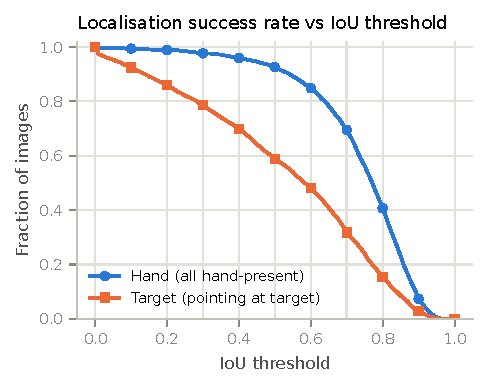
\includegraphics[width=0.48\linewidth]{figures/results/iou_success_rate}
  \caption{Share of test images whose hand or target box reaches each IoU threshold.}
  \Description{Two curves of success rate against IoU threshold; the hand curve stays above 0.9 up to IoU 0.5 and falls after 0.7, while the target curve falls steadily, reaching 0.59 at IoU 0.5 and 0.32 at 0.7.}
  \label{fig:curves}
\end{figure}

\begin{figure}[h]
  \centering
  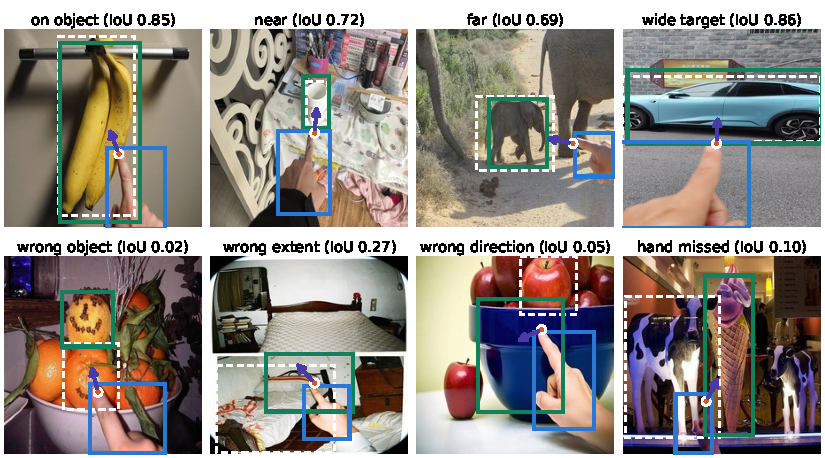
\includegraphics[width=\linewidth]{figures/qualitative}
  \caption{Successes (top) and failures (bottom) on EgoPoint test images: predicted hand (blue), fingertip and direction, and target (green); labelled target dashed. Bottom row, one example per failure type of Section~\ref{sec:failures}.}
  \Description{Eight egocentric images. Top row: correct target boxes for bananas touched by the finger, a cup near the finger, a young elephant far from the finger, and a car. Bottom row: a box on the wrong orange in a bowl of oranges, a box on part of a bed instead of the labelled bed, a box on a bowl while the label is an apple above it, and a frame where the hand gate missed the hand.}
  \label{fig:qual}
\end{figure}
